\subsection{NATaS : ordonnancer des tâches sur une machine NUMA}
Ne trouvant pas de solution adaptée à notre besoin, nous avons créer notre propre ordonnanceur de tâches.
%
Celui-ci est très basique, il ne prend en compte que l'affinité mémoire des tâches.
%
Pour cela, nous utilisons un container de tâches thread-safe par banc NUMA.
%
Ce container permet à plusieurs threads d'insérer/retirer des tâches en limitant la contention.
%
Le vol de tâche entre container a aussi été implémenter, il existe une option par tâche pour autoriser ou non le vol de tâche.
%
Dans le cas du parallélisme de boucle, une option permettant de donner une tâche spécifiquement à un thread a été implémentée.


NATas fourni aussi une api permettant de gérer les allocations mémoires et leurs placements.
%
Il permet de faire différents types d'allocations tel que :
\begin{itemize}
  \item distribuer régulièrement la mémoire;
  \item entrelacer les pages mémoires;
  \item bind memory pages.
\end{itemize}
%
Ces allocations font miroir au différent type d'ordonnancements.
%
Dans le cas d'un parallélisme de boucle avec un distribution statique, on distribura la mémoire régulièrement.
%
Dans le cas d'un graphe de tâche, le programmeur donnera la position souhaitée des tâches.
%
Il lui suffira de simuler l'exécution du code, de désactiver le vol de tâches et d'appeler la fonction de migration des pages dans chaque tâche.



NATaS s'interface avec Taggre pour améliorer les performances sur des machines NUMA.
%
La connaissance complète du graphe de tâche permet des améliorations notables sur la distribution mémoire.
%
Comme le graphe sera déroulé de haut en bas lors de son exécution, il parait naturel de distribuer les tâches par hauteur.
%
En supposant que les tâches produisent des données et que ces données sont passées en paramètre aux tâches successeurs dans le graphe, on peut essayer d'optimiser le placement NUMA.
%
Dans un premier temps, on va équilibrer la distribution des tâches sur les bancs NUMA en attribuant une affinité NUMA aux tâches.
%
Cette affinité sera choisie en fonction de la hauteur de la tâche dans le graphe et des affinités NUMA de ses prédécesseurs.
%
Le but étant d'avoir à hauteur fixée, un nombre égale de tâche par banc NUMA tout en minimisant les accès en lecture distant.



%   (-_-)   %
\begin{figure}[t!]
  \centering
  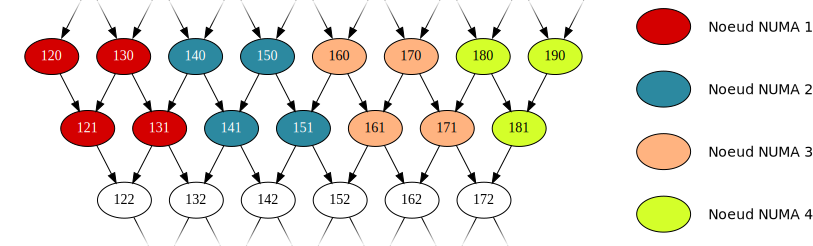
\includegraphics[width=\textwidth]{numa_distrib_example}
  \caption{Exemple de l'algorithme de distribution des tâches en action, la couleur des tâches détermine leurs affinités NUMA. Les tâches en blanches ne sont pas encore traitées.}
  \label{fig:numa_distrib_example}
\end{figure}
